\section*{Introduction}
\begin{wrapfigure}{r}{0.35\textwidth} % r for right, 0.5\textwidth for half the text width
    \centering
    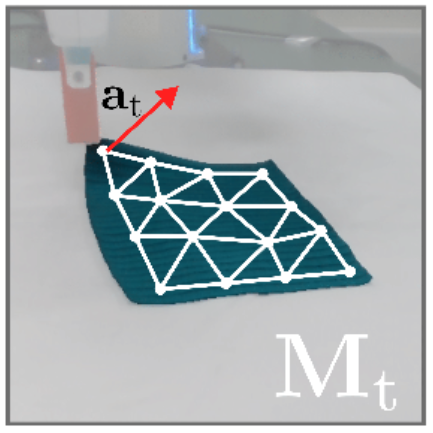
\includegraphics[width=0.35\textwidth]{images/mesh.png} % adjust width of image inside the wrapfigure
    \caption{Vision-based cloth manipulation with mesh privileged information for sample-efficient imitation learning.}
\label{}
\end{wrapfigure}

Recent advancements in imitation learning have demonstrated significant progress in acquiring manipulation skills from human demonstrations~\cite{zhao2024aloha}. A key factor in this success is the adoption of diffusion models, state-of-the-art architectures that effectively learn the distribution of the demonstrated data and show robustness to multimodal data distributions. However, despite their success, these models often require a large number of demonstrations and tend to struggle with visual disturbances in real-world applications~\cite{ze20243d}.

Recent advances have explored 3D representations to improve sample efficiency in imitation learning, as 3D data tends to be more robust to visual noise and facilitate sim-to-real transfer~\cite{ke20243d}. While these approaches have been proven successful for rigid objects, they fall short when applied to deformable objects. Deformables present unique challenges due to their high-dimensional state spaces and self-occlusions, which often lead to ambiguities in visual and 3D representations. A way to overcome these challenges is to have more structured representations, such as graphs, but real-time tracking of graphs remains computationally demanding~\cite{longhinicloth}.

This project seeks to improve the sample efficiency of image-based diffusion policies by incorporating graph-based representations as privileged information during training. By doing so, we hypothesize that diffusion models will require fewer demonstrations and achieve higher sample efficiency. Our approach involves training diffusion models using both visual data and graph-based representations of deformable objects. During testing, the model will be designed to perform without the graph information, relying solely on visual input, thus improving computational efficiency. %The hypothesis is that by training diffusion models with privileged graph representations will improve sample efficiency in learning manipulation skills for deformable objects.

The main contributions of this work would be:
\begin{itemize}
    \item Leveraging graph representations as privileged information during the training of diffusion models to improve sample efficiency for learning manipulation skills of deformable objects.
    \item Designing a policy architecture integrating both visual observations and privileged graph information during training which is robust to missing graph information during testing.
\end{itemize}


\section*{Goal and Objectives}

The goal of this project is to develop a sample-efficient method for learning imitation policies for deformable object manipulation by leveraging privileged information during training. Specifically, we aim to design a diffusion-based policy that is robust to missing graph information during testing, improving computational efficiency without sacrificing performance. If the results are positive, we expect to publish this work in a top-tier robotics or machine learning conference.
Your task will be to:
\begin{itemize}
    \item Conducting a thorough literature review to identify gaps in current research on imitation learning for rigid and deformable object manipulation.
    \item Familiarizing with tools already available in our robotics lab such as frameworks integrating diffusion models for imitation learning and frameworks for graph tracking, such as Gaussian Splatting, both in simulation and the real world.
    \item Implementing baseline models and collecting demonstration datasets in both simulated and real environments.
    \item Testing and evaluating the proposed hypothesis by comparing the performance of models trained with and without privileged graph information.
    \item Report the results in a scientific manner.
\end{itemize}

\section*{Requirements}

This project is suitable for students interested in the field of robotics and machine learning. You should have strong programming skills in any high-level language (Python, C++, Julia, etc.. ). Some basic knowledge about ROS is fundamental, and some experience with training machine learning models is needed. Desirable skills include knowledge knowledge of / experience with robotic manipulation, optimizing code for speed and parallelism, and experience with robotic hardware.